\documentclass[a4 paper, 12 pt]{article}  
	\usepackage[utf8]{inputenc}
	\usepackage[french]{babel}
	\usepackage{color}
	\usepackage{hyperref}
	\usepackage{graphicx}
	\usepackage[table]{xcolor}
	\usepackage{authblk}
	\usepackage{perpage}
	\usepackage{enumitem}
	
	\author[1]{Daril Yousfi \thanks{Contact auteur: \texttt{daril.yousfi@etud.univ-pau.fr}} \and {Robin Florian \thanks{Contact auteur: \texttt{florian.robin@etud.univ-pau.fr}}}}
	
	\title{Cloud Computing}
	\date {} 
	\MakePerPage{footnote}
	\frenchbsetup{StandardLists=true}

\begin{document}

\maketitle

\tableofcontents

\listoffigures

\listoftables

\newpage

\begin{abstract}
Le cloud computing est l’accès à des ressources informatiques sur demande par l’intermédiaire d’un réseau. C’est un service destiné au client qui permet d’utiliser différentes ressources en fonction de ses besoins à la place de tout installer sur sa machine. On peut distinguer plusieurs types de services, il y a notamment le service privé, partagé et public. Tous ses services peuvent être utilisables sous forme hybride. \newline

Le service peut aussi proposer différentes solutions à l’utilisateur comme le calcul, le stockage, le back-up, l’utilisation de bande passante (IaaS), une plateforme d’exploitation (PaaS). Cela permet à l’utilisateur de disposer de grands moyens techniques comme des applications et logiciels (Saas) en contrepartie d’une rémunération du service qui dépend seulement du besoin. Certains des services sont également gratuits grâce aux publicités.
\end{abstract}

 \section{Introduction}

\begin{itemize}[label=\textbullet] 

\item \textbf{Définition}
\newline 

Voici une définition\footnote{remarque : cette définition n'est pas universelle, elle dépend uniquement de l'avis de chercheurs.} :

« Le cloud computing est un modèle Informatique qui permet un accès facile et à la demande par le réseau à un ensemble partagé de ressources informatiques configurables (serveurs, stockage, applications et services) qui peuvent être rapidement provisionnées et libérées par un minimum d’efforts de gestion ou d’interaction avec le fournisseur du service » \cite{barkat2018composition}  \newline


Il existe différents types de services proposés par le cloud computing :
\begin{itemize}
\item SaaS (Software as a Service)
\item le PaaS (Platform as a Service) 
\item IaaS (Infrastructure as a Service)
\item MBaaS (Mobile Backend as a Service)
\end{itemize}
\vspace{1cm}


On distingue généralement trois types de cloud :
  
\begin{enumerate}
\item le cloud public (accessible par Internet)
\item le cloud d'entreprise ou privé (accessible uniquement sur un réseau privé.) 
\item le cloud intermédiaire ou hybride (mix entre le cloud public et le cloud privé.)
\end{enumerate}

\end{itemize}


\section{Les débuts du cloud computing}

Les premières apparitions du cloud computing datent des années 1950, tout était accessible par des terminaux en utilisant des mainframe. John Mc Carthy\footnote{John McCarthy est le pionnier du cloud computing, il est le premier à créer un système de partage sur un ordinateur avec plusieurs utilisateurs connectés ensemble.} Il a donc émis l’idée d’accéder seulement aux services du mainframe en 1961. 
Cette idée a commencé à s’ébruiter après l’apparition d’internet en 1980, cependant 10 ans plus tard le concept est proposé mais ne rencontre aucun succès. Ce n’est que vers les années 2000 avec l’émergence des hébergeurs web que le terme « cloud computing » \cite{WikiHistoire} et son concept ont été adoptés.  \newline 

Les premiers services proposés au grand public correspondaient au courrier électronique, des outils collaboratifs, le CRM\footnote{Customer Relationship Management, cela correspond à une stratégie de gestion et intéractions d'une entreprise.} et les environnements de développement et de test.

Vers 2010, \cite{WikiHistoire} le succès du cloud computing a commencé à se ressentir car l’accès à internet a été déployé de manière massive. De plus les équipements informatiques et la puissance des machines ont également augmenté ce qui a permis de plus facilement mettre le cloud computing en place. En effet plusieurs améliorations ont été effectuées comme : 
\begin{itemize}

	 \item l’augmentation de la puissance des serveurs 
	 \item a performance des processeurs a été accru
	 \item les coûts de stockages ont été largement réduits

\end{itemize}
\vspace{0.5cm}


 Cela a permis une baisse considérable du prix des services proposés par les hébergeurs internet. Ainsi les entreprises comme les particuliers peuvent utiliser les services à partir d’une infrastructure dirigé par un fournisseur. Toutes les données sont en ligne et ne sont plus stockées sur les disques dur des ordinateurs. Néanmoins en 2009 seuls $10\%$  des entreprises utilisaient le cloud computing au vue de la complexité de la mise en place de ce système. De nos jours, avec l’avancée technologique, cela est beaucoup plus simple de mettre en place ce genre de système.


\section{Les différents services proposés }


\begin{figure} [h] 
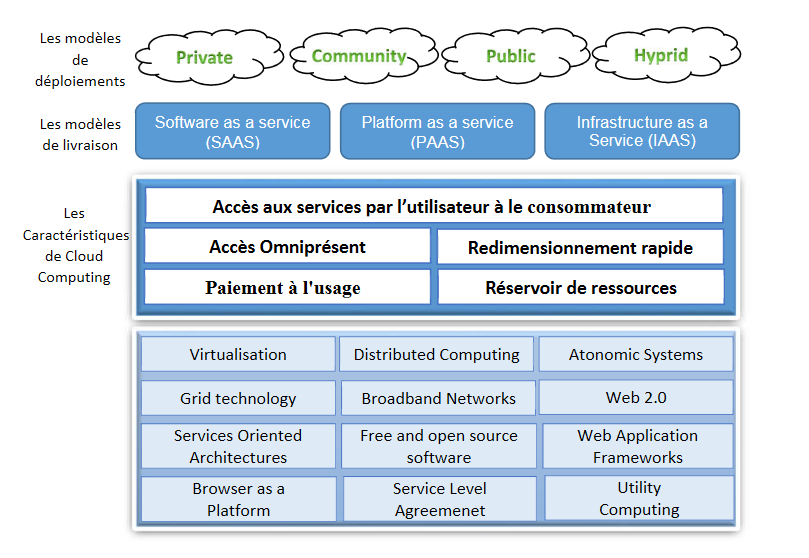
\includegraphics[scale=0.5]{CP2.png} 
\caption{ Le cloud Computing en une image \cite{barkat2018composition}}
\label{1}
\end{figure}

\begin{itemize}

\item Software as a service (SaaS) : Ce service est celui où le fournisseur contrôle le plus les ressources informatiques, en effet l’utilisateur ne gère que la couche application. Toutes les autres couches (données, équipements, réseau, machine virtuelle, etc…) sont donc gérées par le fournisseur. L’utilisateur peut donc accéder à une application par le biais d’un réseau internet. Cela évite d’installer les différents logiciels sur les machines des clients ainsi que d’effectuer régulièrement les mises à jour car celles-ci sont faites par le fournisseur. Les applications les plus fréquentes sont les solutions CRM et de messagerie mais il en existe d’autres comme :  les réseaux sociaux, la finance, les ventes, les solutions bureautiques, contrôle de gestion, etc… \newline

\item Platform as a service (PaaS) : Dans ce service l’utilisateur à accès à l’application aux données et au moteur d’exécution. Il utilise donc une plateforme d’exécution gérée et mis en place sur le cloud où il peut déployer des applications développées par ses propres soins ou récupérer sur internet. Par exemple oracle est un environnement pour les développeurs où ils peuvent programmer en Java sans se soucier de la partie réseau, serveurs et système d’exploitation. De plus ce type de plateforme met à dispositions des IDE\footnote{integrated development environnement est l'ensemble d'outils mis à disposition pour programmer dans un langage spécifique.} ou SDK\footnote{Sotfware Development Kit désigne l'ensemble des outils pour créer un logiciel.} qui sont des outils largement répandus. \newline

\item Infrastructure as a service (IaaS) : seul le réseau, les serveurs, et les machines virtuelles sont gérés par le fournisseur.\cite{leon:tel-01138912} En effet ce service met à dispositions des utilisateurs ou clients des serveurs, des réseaux et des solutions de stockage en ligne. Le fournisseur met donc à disposition un centre de données qu’il met en place comme bon lui semble ainsi que différents logiciels. Grâce à ce service les utilisateurs peuvent développer des PaaS ou SaaS. L’IaaS est très utilisé pour la puissance de calcul, la sauvegarde et récupération, le management des services et le stockage.(\textbf {voir figure \ref{2})} \newline

\end{itemize}


\section{ L’utilisation du cloud computing }
 \subsection{Pour les entreprises}
 
 Pour comprendre rapidement pourquoi les entreprises utilisent ou pas le cloud computing, voici un récapitulatif (\textbf {voir tableau \ref{3}).}
 \newline
 
 Les entreprises utilisent le cloud computing (privé / hybride) par rapport à son déploiement rapide, en effet une majorité de services sont disponibles et personnalisables facilement. De plus les maintenances sont automatisées par le fournisseur ce qui permet de gagner du temps pour l’entreprise concernée. Le cloud computing offre également un niveau de sûreté accrue (\textbf {voir figure \ref{4})}. En revanche certaines entreprises restent assez opposées par l’utilisation du cloud computing soit pas choix ou par obligation. En effet l’entreprise qui utilise ces services doit avoir une très bonne connexion internet pour exploiter les ressources informatiques. D’autres entreprises font le choix de stocker leurs données à leur manière plutôt que de les mettre sur une plateforme en ligne où elle ne connaît même pas le lieu de stockage \cite{chaoui2016entreprise}. De plus à court terme ce procédé est intéressant mais à moyen terme ou plus, il peut s’avérer que les services du cloud computing deviennent bien plus coûteux que l’hébergement en interne d’une application.
 
 \begin{figure} [h]
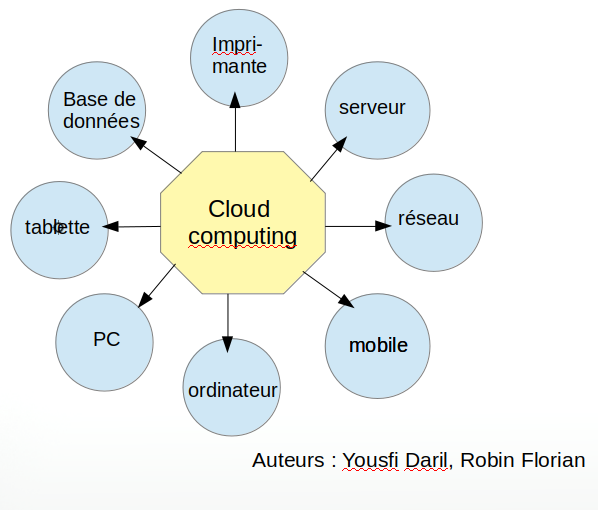
\includegraphics[scale=0.7]{schemaCreer.png}
\caption{Les domaines d'application pour les entreprises.}
\label{4}
\end{figure}
 
\subsection{Pour les utilisateurs privées}

Ce type de client utilise généralement le cloud computing dit public ou hybride. Comme pour les entreprises ce service permet de réaliser des économies à court terme par exemple beaucoup de personnes stockent leurs données sur diverses applications de stockage très connues. Beaucoup de personnes de personnes utilisent les environnements pour programmer pendant leur temps libre aussi. Le public utilise largement les services de courrier électronique, de gestion de documents ou bien de services liés à la finance. Les utilisateurs de tout ces services ont aussi conscience que leurs données peuvent être partagés où collecter par des organismes tiers où la juridiction est différente de celle du pays de l’utilisateur. 
 

 
\begin{figure} 
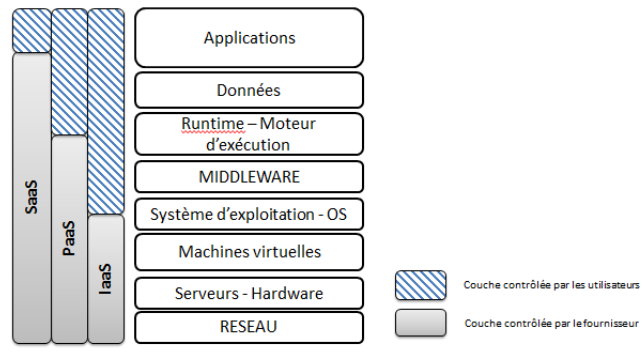
\includegraphics[scale=0.9]{CP1.png}
\caption{Les différentes couches partagées \cite{leon:tel-01138912}}
\label{2}
\end{figure}

\clearpage

\section{Avantages et inconvénients}

\begin{table}[h] 
\rowcolors{1}{gray}{lightgray}
\begin{tabular} {|p{7cm}||p{7cm}|} \hline
	\textcolor{white}{\textbf{Avantages}} & \textcolor{white}{\textbf{Inconvénients}} \\ \hline
 \textcolor{white}{Un fonctionnement simplifié pour tous.} &\textcolor{white}{Risque de sécurité avec des attaques informatiques.}\\ \hline
 
 \textcolor{white}{La maîtrise du budget.} & \textcolor{white}{On dépend d’un fournisseur d’accès.}\\ \hline

\textcolor{white}{La sécurité des données garanties en fonction du fournisseur.} &\textcolor{white}{ Bande passante importante nécessaire.}\\ \hline

\textcolor{white}{Une grande flexibilité des services.} &\textcolor{white}{ Perte de maîtrise d’une partie du système informatique.} \\ \hline

\textcolor{white}{Support idéal pour le travail collaboratif.} & \textcolor{white}{Impact environnemental négatif.} \\ \hline 

\textcolor{white}{Technologie de pointe mis en œuvre.} & \textcolor{white}{Risque d’utilisation des données par des organismes tiers.} \\ \hline



\end{tabular}
\caption{ Le cloud computing, un bon choix ? \cite{chaoui2016entreprise}}
\label{3}
\end{table}


\section{Critiques et limites du cloud computing }

Certaines personnes célèbres dans le milieu de l’informatique critiquent ouvertement le cloud computing. En effet c’est le cas de Richard Stallman, fondateur de la Free Software Foundation qui pense que le cloud computing ne mérite pas son succès. De son point de vue les sociétés qui gèrent toutes ces données ont un risque d’en perdre le contrôle. Il a déclaré que : « le cloud computing pose un sérieux danger. Les entreprises et les individus perdent le contrôle direct sur leurs données en les confiant à des tiers ». \cite{CCTH} Toujours selon lui, il pense qu’il est préférable que les utilisateurs stockent leurs données personnelles eux-mêmes plutôt que de faire confiance à des fournisseurs où la protection et la privatisation des données n’est pas forcément garanti à $100\%$.\newline 

En effet si le développeur du logiciel le désir il peut accéder à toutes les informations des utilisateurs. Ces applications sont donc hors de portée des utilisateurs. Il dit également que le cloud computing n’est pas une option économique viable sur le long terme et que les utilisateurs ont tout intérêt à administrer leur système de stockage eux-mêmes. Larry Ellison, patron d’Oracle avait lui aussi critiqué le cloud computing vers 2010. 

\newpage

\bibliographystyle{plain}
\bibliography{mabiblio}

\end{document}